\documentclass[tikz,border=2pt]{standalone}
\usepackage{amsmath,amssymb}
\usepackage{tikz}
\usetikzlibrary{arrows.meta}

\begin{document}
% A surplus variable turns a >= requirement into an equation: it measures by how much the
% requirement is exceeded (diet problem, calorie constraint x_A + 2 x_B >= 6).
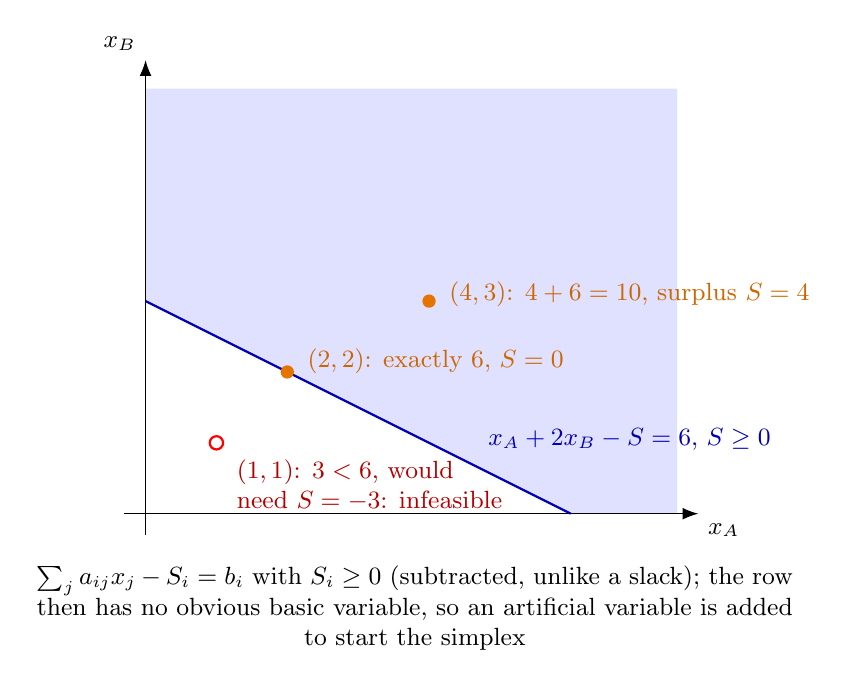
\begin{tikzpicture}[x=0.9cm, y=0.9cm, every node/.style={font=\small}, >={Latex[length=2mm]}]
	\fill[blue!12] (6,0) -- (7.5,0) -- (7.5,6) -- (0,6) -- (0,3) -- cycle;
	\draw[->] (-0.3,0) -- (7.8,0) node[below right] {$x_A$};
	\draw[->] (0,-0.3) -- (0,6.4) node[above left] {$x_B$};
	\draw[blue!70!black, thick] (6,0) -- (0,3);
	\node[blue!70!black, font=\small, anchor=south west] at (4.7,0.75) {$x_A+2x_B-S=6$, $S\ge0$};
	\fill[orange!90!black] (4,3) circle (2.4pt);
	\node[orange!80!black, font=\small, anchor=west] at (4.15,3.1) {$(4,3)$: $4+6=10$, surplus $S=4$};
	\fill[orange!90!black] (2,2) circle (2.4pt);
	\node[orange!80!black, font=\small, anchor=west] at (2.15,2.15) {$(2,2)$: exactly $6$, $S=0$};
	\draw[red, thick] (1,1) circle (2.4pt);
	\node[red!70!black, font=\small, anchor=north west, align=left] at (1.15,0.9) {$(1,1)$: $3<6$, would\\ need $S=-3$: infeasible};
	\node[anchor=north, align=flush center, text width=9.6cm] at (3.8,-0.6) {$\sum_ja_{ij}x_j-S_i=b_i$ with $S_i\ge0$ (subtracted, unlike a slack); the row then has no obvious basic variable, so an artificial variable is added to start the simplex};
\end{tikzpicture}
\end{document}
